%%*****************************************************************************
%% $Id$
%%*****************************************************************************
%% Author: Gerd Neugebauer
%%-----------------------------------------------------------------------------
\documentclass{extex-doc}

\usepackage{makeidx}

\title{\ExTeX\ User's Guide}
\author{Gerd Neugebauer}

\newcommand\Arg[1]{\(\langle\){\tt\itshape #1}\(\rangle\)}
\newcommand\CLI[1]{\texttt{-#1}\index{#1@\texttt{-#1}}}
\newcommand\Property[1]{\texttt{#1}\index{#1@\texttt{#1}}}
\newcommand\File[1]{\texttt{#1}\index{#1@\textsf{#1}}}
\newcommand\Prog[1]{\texttt{#1}\index{#1}}
\newcommand\Mode[1]{\texttt{#1}\index{#1}}
\newcommand\macro[1]{\texttt{\char`\\#1}\index{#1@\texttt{\char`\\#1}}}
\newcommand\Macro[1]{\texttt{\char`\\#1}}
\newcommand\tag[1]{\(\langle\)\textit{#1}\(\rangle\)}

\newenvironment{syntax}{\vspace{-\parskip}%
  \begin{tabbing}\kern2em\=\kern2em\=\kill}{\end{tabbing}}
\newenvironment{pre}{\par\begingroup\small\tt\obeylines\obeyspaces}{\endgroup\par}

\def\setVersion$#1: #2.#3${\gdef\Version{0.#3}}
\setVersion$Revision$

\providecommand\indexGroup[1]{\vskip 12pt plus 4pt minus 2pt
  \textbf{\sffamily\normalsize #1}%
  \vskip 6pt plus 3pt minus 1pt
  \nopagebreak
}
\makeindex

\usepackage{ragged2e}
\newenvironment{primitives}{\begin{quotation}\noindent\small}{\end{quotation}}

\begin{document}%%%%%%%%%%%%%%%%%%%%%%%%%%%%%%%%%%%%%%%%%%%%%%%%%%%%%%%%%%%%%%%

\begin{titlepage}
  \parindent=0pt
  \begin{center}
  \vspace*{1pt}
  \vfill
  \ExTeXbox
  %
\includegraphics[width=\textwidth]{img/ExTeX-splash}
  \vfill
  \textsf{\bfseries\Huge User's Guide}
  \vfill
  \textsf{\Large Version \Version}
  \vfill
  \textsf{\large Gerd Neugebauer}
  \vfill
  \vfill
%\maketitle

  \begin{abstract}\noindent
    This document describes \ExTeX. It explains how to get \ExTeX\ up
    and running and which features \ExTeX\ offers to you. Since
    \ExTeX\ provides a testbed for experimentation the focus has been
    put on the default configurations.

    The intended audience for this document are end users of the
    typesetting engine who want to use \ExTeX\ on the command line or
    as replacement of \TeX.
  \end{abstract}
  \unitlength=1mm
  \begin{picture}(0,0)
    \put(56,116){\makebox(0,0){\scalebox{6}{\rotatebox{45}{\color{red}\textsf{\Huge\bfseries Draft}}}}}
  \end{picture}
  \end{center}
\newpage
\footnotesize
\copyright\ 2005 The \ExTeX\ Group and individual authors listed below 

Permission is granted to copy, distribute and/or modify this document
under the terms of the GNU Free Documentation License, Version 1.2 or
any later version published by the Free Software Foundation. A copy of
the license is included in the section entitled ``GNU Free
Documentation License''.

\vfill

Gerd Neugebauer\\
Im Lerchelsb\"ohl 5\\
64521 Gro\ss-Gerau (Germany)
\smallskip

Net: \href{mailto://gene@gerd-neugebauer.de}{gene@gerd-neugebauer.de}

\end{titlepage}

\tableofcontents

%------------------------------------------------------------------------------
\chapter{Introduction}
%@author Gerd Neugebauer

\ExTeX{} aims at providing a high-quality typesetting system. The
development of \ExTeX\ has been inspired by the experiences with \TeX.
The focus lies on an open design and a high degree of configurability.
Thus \ExTeX\ should be a good base for further development.

On the other hand we have to take care not to leave the current user
base of \TeX\ behind. pdf\TeX\ has taught us that a migration path
from \TeX\index{TeX@\TeX} has a positive value in it. In the mean time
the majority of \TeX\ users applies in fact
pdf\TeX\index{pdfTeX@pdf\TeX}.

To provide a backward compatibility of \ExTeX\ with
\TeX\index{TeX@\TeX} one special configuration is provided. Thus
backward compatibility is just a matter of configuration.


\section{This Document}

This document is meant to be a reference document. It should contain
all information neccesary to know. It is not meant ot be a tutorial.
Thus do not expect tutorial type materaial in this document.


\section{Web Site}
%@author Gerd Neugebauer

There is a web site devoted to \ExTeX. \index{WWW}\index{Web Site}This
web site can be reached via the URL

\begin{quotation}
  \url{http://www.extex.org}
\end{quotation}


\section{Mailing Lists}
%@author Gerd Neugebauer

If you are ready to try \ExTeX{} you might as well want to join a
mailing list to get in contact with the community.\index{Mailing list}

\begin{quotation}
  \url{http://www.dante.de/listman/extex}
\end{quotation}


\section{Reporting Bugs}
%@author Gerd Neugebauer


If you find any bugs in \ExTeX\ you can submit them either via a HTML
form or via email. You can find the HTML form at
\begin{quotation}
  \url{http://www.extex.org/bugs}
\end{quotation}
Emails containing the description can be sent to
\begin{quotation}
  \href{mailto:extex-bugs@dante.de}{extex-bugs@dante.de}
\end{quotation}

Please include in your description 
\begin{itemize}
\item the source of a \emph{minimal} example showing the problem
\item the log file resulting from running this example
\item a description why you think that something went wrong and what
  the expected result would be
\item a description of the environment you are using (host
  architecture, operating system, Java version)
\end{itemize}


%------------------------------------------------------------------------------
\chapter{Getting Started}
%@author Gerd Neugebauer

In this chapter we describe the steps you can take to get \ExTeX\ up
and running. We try to use as few as possible premises. Thus it should
be not too hard to get started.

\section{Prerequisites}
%@author Gerd Neugebauer

\subsection{Java}
%@author Gerd Neugebauer

You need to have Java 1.4.2\index{Java} or later installed on your
system. You can get Java for a several systems directly from
\url{java.sun.com}. Download and install it according to the
installation instructions for your environment.

To check that you have an appropriate Java on your path you can use
the command \texttt{java} with the argument \texttt{-version}. This
can be seen in the following listing:

\lstset{morecomment=[l]{\#}}%
\begin{lstlisting}{morecomment=[l][keywordstyle]{>}}
# java -version
java version "1.4.2_06"
Java(TM) 2 Runtime Environment, Standard Edition (build 1.4.2_06-b03)
Java HotSpot(TM) Client VM (build 1.4.2_06-b03, mixed mode)
#
\end{lstlisting}


\subsection{TEXMF}
%@author Gerd Neugebauer

If you want to use more than the pure \ExTeX\ engine, fonts and macros
can be inherited from a texmf tree\index{texmf}. \ExTeX\ itself does
not contain a full texmf tree. It comes just with some rudimentray
files necessary for testing. Thus you should have installed a texmf
tree, e.g. from a \TeX Live\index{TeXlive@\TeX Live} installation.
This can be found on the \href{http://www.ctan.org}{Comprehensive
  \TeX\ Archive Network (CTAN)}\index{CTAN}.

There is no need to install the texmf tree in a special place. You
have to tell \ExTeX\ anyhow where it can be found. It is even possible
to work with several texmf trees.

One requirement for the texmf trees is that they have a file database
(\File{ls-R}). \ExTeX\ can be configured to work without it, but then
\ExTeX\ is deadly slow. Thus you do not really want to try this
alternative.


\section{Getting \ExTeX}
%@author Gerd Neugebauer

\subsection{Getting the Installer}
%@author Gerd Neugebauer

The simplest way to get \ExTeX\ up and running is to use the \ExTeX\ 
installer. This installer\index{installer} is distribted as one file
\File{ExTeX-setup.jar}. You can download it from

\begin{quotation}
  \url{http://www.extex.org/download/}
\end{quotation}

\INCOMPLETE


\subsection{Getting the Sources}
%@author Gerd Neugebauer

The sources of \ExTeX\ are stored in a CVS repository. To access this
repository you need access to the internet and CVS installed in some
way.

The coordinates of the repository are:\index{repository}\index{CVS}
\medskip

\begin{tabular}{ll}\toprule
  Connection type: & \texttt{pserver}			\\
  User:		   & \texttt{anonymous}			\\
  Host:		   & \texttt{cvs.extex.berlios.de}	\\
  Location:	   & \texttt{/cvsroot/extex}		\\
  Module:	   & \texttt{ExTeX}			\\\bottomrule
\end{tabular}
\bigskip

We assume here that you have access to CVS on the command line. This
can be either a shell on a Unix-like system or somethng like cygwin on
Windows. We also assume that you have direct connection to the internet.

First we create a directory where the sources are stored:
\begin{lstlisting}{}
# mkdir ExTeX
\end{lstlisting}

Next we change the current directory to this base directory:
\begin{lstlisting}{}
# cd ExTeX
\end{lstlisting}

Now we log into the CVS repository. This login uses an anonymous
account. This enables us to download the sources but not to commit any
changes. The committing is restricted to members of the \ExTeX{} team.
\begin{lstlisting}{}
# cvs -d:pserver:anonymous@cvs.extex.berlios.de/cvsroot/extex login
\end{lstlisting}

Finally we can check out the sources:
\begin{lstlisting}{}
# cvs -d:pserver:anonymous@cvs.extex.berlios.de/cvsroot/extex co ExTeX
\end{lstlisting}

This command shows a lot of output. At the end the current directory
is filled with a lot of files and directories.

\section{Installing \ExTeX}
%@author Gerd Neugebauer

There are several ways to install \ExTeX. Some of them are described
in this section. 

\subsection{Installing \ExTeX\ with the Installer}\label{sec:installer}
%@author Gerd Neugebauer

\begin{figure}[tp]
  \centering
  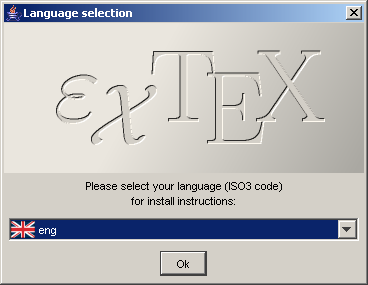
\includegraphics[width=.8\textwidth]{img/inst1}
  \caption{The Language Selection in the Installer}
  \label{fig:inst1}
\end{figure}
The easiest installation of \ExTeX\ works with the \ExTeX\ installer.
This installer is named \File{ExTeX-setup.jar}. You can start the
installer with the following command line:\index{installer}

\begin{lstlisting}{}
# java -jar ExTeX-setup.jar
\end{lstlisting}

On Windows\index{Windows} with a properly installed Java\index{Java}
you can also start the installer by double-clicking
\texttt{ExTeX-setup.jar} in the Explorer\index{Explorer}.

The installer provides a graphical user interface with a wizard
guiding you through the installation process. The first dialog is
shown in figure~\ref{fig:inst1}. As you can see you can select one of
several languages for the installation process. Currently the
languages English and German are supported. There might be some more
at the time you are performing the
installation.\index{installer!language}\index{language!installer}

Note that the internationalization covers the installer only. \ExTeX\
can be run under different language environments as well. This is
controlled by a setting at run-time. Currently only an English
language binding for \ExTeX\ is provided.\index{language}

Finally you have to make sure that the executables \Prog{extex} or
\Prog{extex.bat} is on your path for executables.\index{path}


\subsection{Replaying an Installation}
%@author Gerd Neugebauer

Sometimes it is desirable to perform an installation on several
similar machines. This means that the answers to the questions in the
installer are the same. This process can be automated.
\begin{figure}[tp]
  \centering
  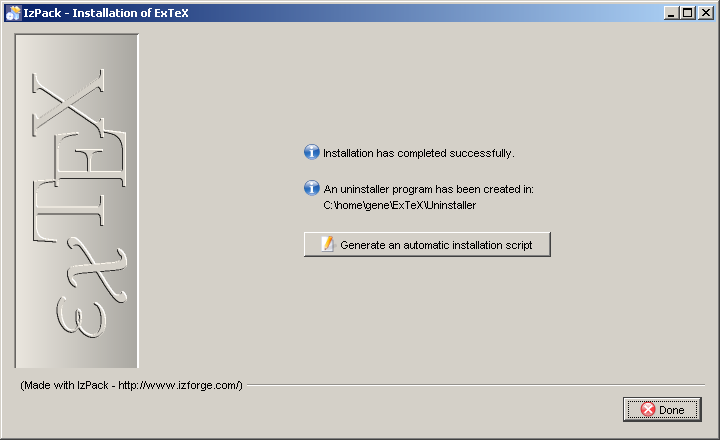
\includegraphics[width=.8\textwidth]{img/inst8}
  \caption{Generating a Auto-Configuration for the Installer}
  \label{fig:inst8}
\end{figure}

In figure~\ref{fig:inst8} you can see the last screen of the
installer. Here you have the possibility to select the button
``Generate an automatic installation script''. This produces an XML
file which can be passed to the installer to avoid the
dialogs.\index{installer}\index{installation script}

Suppose you have named the file \texttt{replay.xml} in the file
selector which pops up when the button has been pressed. Then you can
replay the installation with the following command invocation:

\begin{lstlisting}{}
# java -jar ExTeX-setup.jar replay.xml
\end{lstlisting}

This supposes that the two files \File{ExTeX-setup.jar} and
\texttt{replay.xml} are in the current directory.

Finally you have to make sure that the executables \Prog{extex} or
\Prog{extex.bat} is on your path for executables.\index{path}


\subsection{Creating the \ExTeX\ Installer}
%@author Gerd Neugebauer

You can create the installer of \ExTeX\ from the sources. All you need
for this step is contained in the source distribution. Suppose you are
in the base directory of the distribution. Then the following command
creates the installer:\index{installer!building}

\begin{lstlisting}{}
# build installer
\end{lstlisting}

As a result the file \File{ExTeX-setup.jar} is created in the
directory \texttt{target}. This file is a self-contained installer.
You can immediately start the installer with the following command line:

\begin{lstlisting}{}
# java -jar target/ExTeX-setup.jar
\end{lstlisting}

In addition the installer file can be moved to any other place -- even
other machines -- and run the installation there (see also
section~\ref{sec:installer}).


\subsection{Installing \ExTeX\ from the Sources on the Command Line}
%@author Gerd Neugebauer

To install you can use the build script provided in the \ExTeX{}
base directory.

\begin{lstlisting}{}
# build -Dinstall.dir=/usr/local/share/ExTeX install
\end{lstlisting}

Additionally you have to copy the file \File{.extex} from the base
directory of the \ExTeX\ to your home directory and adapted to your
installation. Most probably the value of the property
\Property{extex.texinputs} needs adaption to point to your
texmf\index{texmf} trees.

Finally you have to make sure that the executables \Prog{extex} or
\Prog{extex.bat} is on your path for executables.

Now you can forget the source directory. It is not needed any more
unless you are debugging or developing \ExTeX{} extensions.


%------------------------------------------------------------------------------
\section{Configuring \ExTeX}
%@author Gerd Neugebauer

The behaviour of \ExTeX\ can be influenced via command line arguments
and configuration files. Most of the times the startup files will be
enough for the casual user.


\subsection{Startup Files}
%@author Gerd Neugebauer

Whenever \ExTeX\ starts it looks for startup files named
\File{.extex}. This file is sought in the user's home directory in
in the current directory. The settings in the current directoy
overwrite the settings from the user's home directory. Those in turn
overwrite the built-in settings.

\ExTeX\ user properties files contain setting of properties. This is
done in a line-based way. Lines containing only whitespace characters
are ignored. If the first character is a hash sign (\verb|#|) then the
line is treated as a comment and ignored.

The first appearance of a equal sign (\verb|=|) or the colon
(\verb|:|) separates the name of the property from the value. Leading
and trailing whitespace is ignored both for the name and the value of
the property.

Some characters have a special meaning. The backslash (\verb|\|) acts
as an escape character. The sequence \verb|\n| is replaced by the
newline character. If the last character in a line is a backslash then
the line is continued in the next line. To produce a single backslash
it has to be doubled.

You can set any property name you like to a legal value. \ExTeX\ will
not complain about unknown peoperties but ignore them silently.
The following properties are used by \ExTeX:

\begin{description}
\item[\Property{extex.code}]\ \\
  This parameter contains \ExTeX\ code to be executed directly. The
  execution is performed after any code specified in an input file.

   Example:\index{relax@\texttt{\char`\\relax}}
\begin{lstlisting}{}
  extex.code = \\relax
\end{lstlisting}

\item[\Property{extex.config}]\ \\
  This parameter contains the name of the configuration resource to
  use. This configuration resource is sought on the classpath.

  Example:
\begin{lstlisting}{}
  extex.config = tex.xml
\end{lstlisting}

\item[\Property{extex.encoding}]\ \\
  This parameter contains the name of the property for the standard
  encoding to use.

  Example:
\begin{lstlisting}{}
  extex.encoding = ISO-8859-1 
\end{lstlisting}

\item[\Property{extex.error.handler}]\ \\
  This parameter contains the logical name of the error handler.

  Example:
\begin{lstlisting}{}
  extex.error.handler = TeX
\end{lstlisting}

\item[\Property{extex.fonts}]\ \\
  This parameter contains the property indicating where to find font
  files. The value is a path similar to \Property{extex.texinputs}.

  Example:
\begin{lstlisting}{}
  extex.fonts = /usr/local/share/fonts
\end{lstlisting}

\item[\Property{extex.halt.on.error}]\ \\
  This boolean parameter contains the property indicating whether
  the processing should stop after the first error. Allowed values are
  \verb|true| and \verb|false|.

  Example:
\begin{lstlisting}{}
  extex.halt.on.error = false
\end{lstlisting}

\item[\Property{extex.file}]\ \\
  This parameter contains the file to read from. It has no default. If
  this property is not set or set to the empty string then no attempt
  is made to read a file. Maybe the user is asked to provide one.

  Example:
\begin{lstlisting}{}
  extex.file = abc.tex
\end{lstlisting}

\item[\Property{extex.fmt}]\ \\
  This parameter contains the name of the format to read. An empty
  string denotes that no format should be read. This is the default.
  In thi case \ExTeX\ acts with no macros or fonts preloaded.

  Example:
\begin{lstlisting}{}
  extex.fmt = plain
\end{lstlisting}

\item[\Property{extex.ini}]\ \\
  If set to \verb|true| then act as ini\TeX. This command line option
  is defined for compatibility to \TeX\ only. In \ExTeX\ it has no
  effect at all. Allowed values are \verb|true| and \verb|false|.

  Example:
\begin{lstlisting}{}
  extex.ini = true
\end{lstlisting}

\item[\Property{extex.interaction}]\ \\
  This parameter contains the interaction mode. possible values are
  the numbers 0\dots3 and the symbolic names \Mode{batchmode} (0),
  \Mode{nonstopmode} (1), \Mode{scrollmode} (2), and
  \Mode{errorstopmode} (3).

  Example:
\begin{lstlisting}{}
  extex.interaction = scrollmode
\end{lstlisting}

\item[\Property{extex.jobname}]\ \\
  This parameter contains the name of the job. It is overwritten if a
  file is given to read from. In this case the basename of the input
  file is used instead. If no file is read in then the default value
  \verb|texput| is used.

  Example:
\begin{lstlisting}{}
  extex.jobname = texput
\end{lstlisting}

\item[\Property{extex.jobname.master}]\ \\
  This parameter contains the name of the job to be used with high
  priority.

  Example:
\begin{lstlisting}{}
  extex.jobname.master = texput
\end{lstlisting}

\item[\Property{extex.lang}]\ \\
  This parameter contains the name of the locale to be used for the
  messages. The value is a two letter ISO language code.  \ExTeX\ can
  be internationalized ust by providing some files with the translated
  strings. Currently only the language English (\verb|en|) is
  supported.

  Example:
\begin{lstlisting}{}
  extex.lang = en
\end{lstlisting}

\item[\Property{extex.nobanner}]\ \\
  This parameter contains a boolean indicating that the banner should
  be suppressed. Allowed values are \verb|true| and \verb|false|.

  Example:
\begin{lstlisting}{}
  extex.nobanner = false
\end{lstlisting}

\item[\Property{extex.output}]\ \\
  This parameter contains the output format. This logical name is
  resolved via the configuration.

  Example:
\begin{lstlisting}{}
  extex.output = pdf
\end{lstlisting}

\item[\Property{extex.outputdir}]\ \\
  This parameter contain the directory where output files should be
  created. The period is interpreted as the current directory. The
  default is the current directory.

  Example:
\begin{lstlisting}{}
  extex.outputdir = .
\end{lstlisting}

\item[\Property{extex.outputdir.fallback}]\ \\
  This parameter contains the property for the fallback if the output
  directory (\Property{extex.outputdir}) fails to be writable.  The
  period is interpreted as the current directory.

  The default is the current directory. Thus you can reset
  \Property{extex.outputdir} and if this directory happens not to be
  writable then the current directory is used to create the log file
  and output files in.

  Example:
\begin{lstlisting}{}
  extex.outputdir.fallback = .
\end{lstlisting}

\item[\Property{extex.progname}]\ \\
  This parameter can be used to overrule the name of the program shown
  in the banner and the version information.

  Example:
\begin{lstlisting}{}
  extex.progname = iniExTeX
\end{lstlisting}

\item[\Property{extex.stacktrace.on.internal.error}]\ \\
  This parameter can be used to force a stacktrace on stdout if an
  internal error is encountered. This is handy for development.
  Allowed values are \verb|true| and \verb|false|.

  Example:
\begin{lstlisting}{}
  extex.stacktrace.on.internal.error = true
\end{lstlisting}

\item[\Property{extex.texinputs}]\ \\
  This parameter contains the additional directories for searching
  \ExTeX\ input files.
  The directories are separated by the system-dependant separator.
  This separator is a colon (\verb|:|) on Unix\index{Unix} and the semicolon
  (\verb|;|) on Windows\index{Windows}.

  Example:
\begin{lstlisting}{}
  extex.texinputs = /home/gene/lib/tex
\end{lstlisting}

\item[\Property{extex.trace.input.files}]\ \\
  This boolean parameter contains the indicator whether or not to
  trace the search for input files.  Allowed values are \verb|true|
  and \verb|false|.

  Example:
\begin{lstlisting}{}
  extex.trace.input.files = false
\end{lstlisting}

\item[\Property{extex.trace.font.files}]\ \\
  This boolean parameter contains the indicator whether or not to
  trace the search for font files.  Allowed values are \verb|true| and
  \verb|false|.

  Example:
\begin{lstlisting}{}
  extex.trace.font.files = false
\end{lstlisting}

\item[\Property{extex.trace.macros}]\ \\
  This boolean parameter contains the indicator whether or not to
  trace the execution of macros.  Allowed values are \verb|true| and
  \verb|false|.

  Example:
\begin{lstlisting}{}
  extex.trace.macros = false
\end{lstlisting}

\item[\Property{extex.trace.tokenizer}]\ \\
  This boolean parameter contains the indicator whether or not to
  trace the work of the tokenizer.  Allowed values are \verb|true| and
  \verb|false|.

  Example:
\begin{lstlisting}{}
  extex.trace.tokenizer = false
\end{lstlisting}

\item[\Property{extex.typesetter}]\ \\
  This parameter contains the name of the typesetter to use. If it is
  not set then the default from the configuration file is used.

  Example:
\begin{lstlisting}{}
  extex.typesetter = default
\end{lstlisting}

\end{description}


\subsection{Configuration Files}
%@author Gerd Neugebauer

Configuration files of another kind contain the assembly instructions
for \ExTeX. Those files can be used to provide additional features in
\ExTeX. 

\INCOMPLETE

\InputIfFileExists{Configurations/configurations}

%------------------------------------------------------------------------------
\section{Running \ExTeX}
%@author Gerd Neugebauer

Currently \ExTeX\ can be run from the command line. In this respect it
is more or less identical to \TeX\ and can be used as a plug-in
replacement.

The following sample show a simple invocation of \ExTeX\ without any
command line arguments.

{\lstset{morecomment=[l]{*}}%
\begin{lstlisting}{}
# extex
This is ExTeX, Version 0.0 (TeX compatibility mode)
**\relax

*\end

No pages of output.
Transcript written on ./texput.log.
\end{lstlisting}}

In this case \ExTeX\ enters interaction with the user and asks for an
input file. This is indicated by the two asterists. We have entered
\macro{relax} here to indicate that we are not willing to pass in a
file name. The \ExTeX\ system asks us to enter some command --
indicted by the single asterisk. Here we have entered \macro{end} to
indicate that we want to finish the processing. Thus \ExTeX\ 
terminates normally.

\INCOMPLETE

{\lstset{morecomment=[l]{*}}%
\begin{lstlisting}{}
# extex plain
This is ExTeX, Version 0.0 (TeX compatibility mode)
(plain Preloading the plain format: codes, registers, parameters, fonts,
more fonts, macros, math definitions, output routines, hyphenation(hyphen))
*\dump
Beginning to dump on file plain.fmt

*\end

No pages of output.
Transcript written on ./plain.log.
\end{lstlisting}}


\subsection{Command Line Parameters}
%@author Gerd Neugebauer

The invocation of the executable \Prog{extex} can be controlled by
large number of command line arguments. Those command line arguments
are described in the following list:

\begin{description}
\item[\Arg{code}]\ \\
  This parameter contains \ExTeX\ code to be executed directly. The
  execution is performed after any code specified in an input file. On
  the command line the code has to start with a backslash. This
  restriction does not hold for the property settings.

  This commad line argument sets the property \Property{extex.code}
  
\item[\Arg{file}]\ \\
  This parameter contains the file to read from. A file name may not
  start with a backslash or an ampercent. It has no default.

  This command line argument sets the property \Property{extex.file}.
  
\item[\CLI{-} \Arg{file}]\ \\
  This parameter terminates the normal processing of arguments. The
  next argument -- if present -- is interpreted as input file. With
  this construction it is possible to process an input file which
  starts with one of the special characters \verb|\| or \verb|&|.

  This command line argument sets the property \Property{extex.file}
  if a file argument is present.

\item[\CLI{configuration} \Arg{resource}]\ \\
  This parameter contains the name of the configuration resource to
  use. This configuration resource is sought on the class path.
  
  This command line argument sets the property \Property{extex.config}.
  
\item[\CLI{copyright}]\ \\
  This command line option produces a copyright notice on the standard
  output stream and terminates the program afterwards.

\item[\tt\&\Arg{format}]\index{\&}
\item[\CLI{fmt} \Arg{format}]\ \\
  This parameter contains the name of the format to read. An empty
  string denotes that no format should be read. This is the default.

  This command line argument sets the property \Property{extex.fmt}.
  
\item[\CLI{debug} \Arg{spec}]\ \\
  This command line parameter can be used to instruct the program to
  produce debugging output of several kinds. The debug output is
  written to the log file. The specification \Arg{spec} is interpreted
  left to right. Each character is interpreted according to the
  following table:

  \begin{tabular}{lp{.4\textwidth}l}\toprule
    \textit{Spec}& \textit{Description}& \textit{See} \\\midrule
    F& 	This specifier contains the indicator whether or not to trace
    the searching for input files. & 	\Property{extex.trace.input.files}\\
    f& 	This specifier contains the indicator whether or not to trace
    the searching for font files.&      \Property{extex.trace.font.files}\\
    M& 	This specifier contains the indicator whether or not to trace
    the execution of macros.&	 	\Property{extex.trace.macros}\\
    T& 	This specifier contains the indicator whether or not to trace
    the work of the tokenizer.& 	\Property{extex.trace.tokenizer}\\
    \bottomrule
  \end{tabular}

  The following example shows a possible invocation with this
  parameter: 
\begin{lstlisting}{}
# extex -debug FfMT abc.tex
This is ExTeX, Version 0.0 (TeX compatibilty mode)
...
\end{lstlisting}
  
\item[\CLI{halt-on-error}]\ \\
  This parameter contains the indicator whether the processing should
  halt after the first error which has been encountered.

  This command line argument sets the property \Property{extex.halt.on.error}.
  
\item[\CLI{help}]\ \\
  This command line option produces a short usage description on the
  standard output stream and terminates the program afterwards.
  
\item[\CLI{ini}]\ \\
  If set to true then act as ini\TeX.\index{initex@init\TeX} This
  command line option is defined for compatibility to
  \TeX\index{TeX@\TeX} only. In \ExTeX\ it has no effect at all.

  This command line argument sets the property \Property{extex.ini}.

  The following example shows a possible invocation with this
  parameter: 
\begin{lstlisting}{}
# extex -ini abc.tex
This is ExTeX, Version 0.0 (TeX compatibilty mode)
...
\end{lstlisting}
  
\item[\CLI{interaction} \Arg{mode}]\ \\
  This parameter contains the interaction mode. possible values are
  the numbers 0\dots3 and the symbolic names \Mode{batchmode} (0),
  \Mode{nonstopmode} (1), \Mode{scrollmode} (2), and
  \Mode{errorstopmode} (3).

  This command line argument sets the property \Property{extex.interaction}.
  
  The following example shows a possible invocation with this
  parameter:
\begin{lstlisting}{}
# extex -interaction batchmode abc.tex
This is ExTeX, Version 0.0 (TeX compatibilty mode)
...
\end{lstlisting}

\item[\CLI{job-name} \Arg{name}]\ \\
  This parameter contains the name of the job. It is overwritten if a
  file is given to read from. In this case the base name of the input
  file is used instead.

  This command line argument sets the property \Property{extex.jobname}.
  
\item[\CLI{language} \Arg{language}]\ \\
  This parameter contains the name of the locale to be used for the
  messages.

  This command line argument sets the property \Property{extex.lang}.
  
\item[\CLI{output} \Arg{format}]\ \\
  This parameter contains the output format. This logical name is
  resolved via the configuration.

  This command line argument sets the property \Property{extex.output}.

  The following example shows a possible invocation with this
  parameter: 
\begin{lstlisting}{}
# extex -output pdf abc.tex
This is ExTeX, Version 0.0 (TeX compatibilty mode)
\end{lstlisting}
  
\item[\CLI{progname} \Arg{name}]\ \\
  This parameter can be used to overrule the name of the program shown
  in the banner and the version information.  The following example
  shows a possible invocation and the resulting output:

\begin{lstlisting}{}
# extex -progname XeTxE -version
This is XeTxE, Version 0.0 (1.4.2_06)
#
\end{lstlisting}

  This command line argument sets the property \Property{extex.progname}.
  
\item[\CLI{texinputs} \Arg{path}]\ \\
  This parameter contains the additional directories for searching
  \ExTeX\ input files.  The directories are separated by the
  system-dependant separator.  This separator is a colon (\verb|:|) on
  Unix\index{Unix} and the semicolon (\verb|;|) on
  Windows\index{Windows}.
  
  This command line argument sets the property
  \Property{extex.texinputs}.
  
\item[\CLI{texmfoutputs} \Arg{dir}]\ \\
  This parameter contains the name of the property for the fallback if
  the output directory fails to be writable.
  
  This command line argument sets the property
  \Property{extex.outputdir.fallback}.
  
\item[\CLI{texoutputs} \Arg{dir}]\ \\
  This parameter contain the directory where output files should be
  created.

  This command line argument sets the property \Property{extex.outputdir}.
  
\item[\CLI{version}]\ \\
  This command line parameter forces that the version information is
  written to standard output and the program is
  terminated.\index{version} The version of \ExTeX\ is shown and the
  version of the Java engine\index{Java} in parentheses. The following
  example shows a possible invocation and the resulting output:

\begin{lstlisting}{}
# extex -version
This is ExTeX, Version 0.0 (1.4.2_06)
#
\end{lstlisting}
\end{description}

Command line parameters can be abbreviated up to a unique prefix --
and sometimes even more. Thus the following invocations are
equivalent:

\begin{verbatim}
  extex -v
  extex -ve
  extex -ver
  extex -vers
  extex -versi
  extex -versio
  extex -version  
\end{verbatim}


\subsection{Creating Formats}
%@author Gerd Neugebauer

\INCOMPLETE


%------------------------------------------------------------------------------
\chapter{Troubleshooting \ExTeX}
%@author Gerd Neugebauer

This chapter contains some hints in the case of trouble.

\section{Why are my files not found?}
%@author Gerd Neugebauer

\ExTeX\ has a configurable search for external resources.

\INCOMPLETE


%------------------------------------------------------------------------------
\chapter{Primitives of \ExTeX}
%@author Gerd Neugebauer

\ExTeX\ defines a lot of primitives. Those primitives are described below.

\InputIfFileExists{Configurations/primitives}


%------------------------------------------------------------------------------
\appendix

%%*****************************************************************************
%% $Id$
%%*****************************************************************************
%% Author: Gerd Neugebauer
%%-----------------------------------------------------------------------------
\chapter{Licenses}%
\index{license|(}%
%---------The file header---------------------------------------------
%\documentclass[a4paper,12pt]{book} % possibilities : report book article , etc.
%
%\usepackage[english]{babel} %language selection
%\usepackage[T1]{fontenc}
%
%\pagenumbering{arabic}
%
%\usepackage{hyperref}
%\hypersetup{colorlinks, 
%           citecolor=black,
%           filecolor=black,
%           linkcolor=black,
%           urlcolor=black,
%           pdftex}
%
%           
%\begin{document}
%---------------------------------------------------------------------
\section{GNU Free Documentation License}
\label{label_fdl}

\begin{multicols}{3}\tiny\sf%\scriptsize

 \begin{center}

   Version 1.2, November 2002

   Copyright \copyright\ 2000,2001,2002  Free Software Foundation, Inc.
 
   \bigskip
 
   51 Franklin St, Fifth Floor, Boston, MA  02110-1301  USA
  
   \bigskip
 
   Everyone is permitted to copy and distribute verbatim copies
   of this license document, but changing it is not allowed.
\end{center}


\begin{center}
{\bf Preamble}
\end{center}

The purpose of this License is to make a manual, textbook, or other
functional and useful document ``free'' in the sense of freedom: to
assure everyone the effective freedom to copy and redistribute it,
with or without modifying it, either commercially or noncommercially.
Secondarily, this License preserves for the author and publisher a way
to get credit for their work, while not being considered responsible
for modifications made by others.

This License is a kind of ``copyleft'', which means that derivative
works of the document must themselves be free in the same sense.  It
complements the GNU General Public License, which is a copyleft
license designed for free software.

We have designed this License in order to use it for manuals for free
software, because free software needs free documentation: a free
program should come with manuals providing the same freedoms that the
software does.  But this License is not limited to software manuals;
it can be used for any textual work, regardless of subject matter or
whether it is published as a printed book.  We recommend this License
principally for works whose purpose is instruction or reference.


\begin{center}
{\bf 1. APPLICABILITY AND DEFINITIONS}
%\addcontentsline{toc}{section}{1. APPLICABILITY AND DEFINITIONS}
\end{center}

This License applies to any manual or other work, in any medium, that
contains a notice placed by the copyright holder saying it can be
distributed under the terms of this License.  Such a notice grants a
world-wide, royalty-free license, unlimited in duration, to use that
work under the conditions stated herein.  The \textbf{``Document''}, below,
refers to any such manual or work.  Any member of the public is a
licensee, and is addressed as \textbf{``you''}.  You accept the license if you
copy, modify or distribute the work in a way requiring permission
under copyright law.

A \textbf{``Modified Version''} of the Document means any work containing the
Document or a portion of it, either copied verbatim, or with
modifications and/or translated into another language.

A \textbf{``Secondary Section''} is a named appendix or a front-matter section of
the Document that deals exclusively with the relationship of the
publishers or authors of the Document to the Document's overall subject
(or to related matters) and contains nothing that could fall directly
within that overall subject.  (Thus, if the Document is in part a
textbook of mathematics, a Secondary Section may not explain any
mathematics.)  The relationship could be a matter of historical
connection with the subject or with related matters, or of legal,
commercial, philosophical, ethical or political position regarding
them.

The \textbf{``Invariant Sections''} are certain Secondary Sections whose titles
are designated, as being those of Invariant Sections, in the notice
that says that the Document is released under this License.  If a
section does not fit the above definition of Secondary then it is not
allowed to be designated as Invariant.  The Document may contain zero
Invariant Sections.  If the Document does not identify any Invariant
Sections then there are none.

The \textbf{``Cover Texts''} are certain short passages of text that are listed,
as Front-Cover Texts or Back-Cover Texts, in the notice that says that
the Document is released under this License.  A Front-Cover Text may
be at most 5 words, and a Back-Cover Text may be at most 25 words.

A \textbf{``Transparent''} copy of the Document means a machine-readable copy,
represented in a format whose specification is available to the
general public, that is suitable for revising the document
straightforwardly with generic text editors or (for images composed of
pixels) generic paint programs or (for drawings) some widely available
drawing editor, and that is suitable for input to text formatters or
for automatic translation to a variety of formats suitable for input
to text formatters.  A copy made in an otherwise Transparent file
format whose markup, or absence of markup, has been arranged to thwart
or discourage subsequent modification by readers is not Transparent.
An image format is not Transparent if used for any substantial amount
of text.  A copy that is not ``Transparent'' is called \textbf{``Opaque''}.

Examples of suitable formats for Transparent copies include plain
ASCII without markup, Texinfo input format, \LaTeX\ input format, SGML
or XML using a publicly available DTD, and standard-conforming simple
HTML, PostScript or PDF designed for human modification.  Examples of
transparent image formats include PNG, XCF and JPG.  Opaque formats
include proprietary formats that can be read and edited only by
proprietary word processors, SGML or XML for which the DTD and/or
processing tools are not generally available, and the
machine-generated HTML, PostScript or PDF produced by some word
processors for output purposes only.

The \textbf{``Title Page''} means, for a printed book, the title page itself,
plus such following pages as are needed to hold, legibly, the material
this License requires to appear in the title page.  For works in
formats which do not have any title page as such, ``Title Page'' means
the text near the most prominent appearance of the work's title,
preceding the beginning of the body of the text.

A section \textbf{``Entitled XYZ''} means a named subunit of the Document whose
title either is precisely XYZ or contains XYZ in parentheses following
text that translates XYZ in another language.  (Here XYZ stands for a
specific section name mentioned below, such as \textbf{``Acknowledgements''},
\textbf{``Dedications''}, \textbf{``Endorsements''}, or \textbf{``History''}.)  
To \textbf{``Preserve the Title''}
of such a section when you modify the Document means that it remains a
section ``Entitled XYZ'' according to this definition.

The Document may include Warranty Disclaimers next to the notice which
states that this License applies to the Document.  These Warranty
Disclaimers are considered to be included by reference in this
License, but only as regards disclaiming warranties: any other
implication that these Warranty Disclaimers may have is void and has
no effect on the meaning of this License.


\begin{center}
{\bf 2. VERBATIM COPYING}
%\addcontentsline{toc}{section}{2. VERBATIM COPYING}
\end{center}

You may copy and distribute the Document in any medium, either
commercially or noncommercially, provided that this License, the
copyright notices, and the license notice saying this License applies
to the Document are reproduced in all copies, and that you add no other
conditions whatsoever to those of this License.  You may not use
technical measures to obstruct or control the reading or further
copying of the copies you make or distribute.  However, you may accept
compensation in exchange for copies.  If you distribute a large enough
number of copies you must also follow the conditions in section 3.

You may also lend copies, under the same conditions stated above, and
you may publicly display copies.


\begin{center}
{\bf 3. COPYING IN QUANTITY}
%\addcontentsline{toc}{section}{3. COPYING IN QUANTITY}
\end{center}


If you publish printed copies (or copies in media that commonly have
printed covers) of the Document, numbering more than 100, and the
Document's license notice requires Cover Texts, you must enclose the
copies in covers that carry, clearly and legibly, all these Cover
Texts: Front-Cover Texts on the front cover, and Back-Cover Texts on
the back cover.  Both covers must also clearly and legibly identify
you as the publisher of these copies.  The front cover must present
the full title with all words of the title equally prominent and
visible.  You may add other material on the covers in addition.
Copying with changes limited to the covers, as long as they preserve
the title of the Document and satisfy these conditions, can be treated
as verbatim copying in other respects.

If the required texts for either cover are too voluminous to fit
legibly, you should put the first ones listed (as many as fit
reasonably) on the actual cover, and continue the rest onto adjacent
pages.

If you publish or distribute Opaque copies of the Document numbering
more than 100, you must either include a machine-readable Transparent
copy along with each Opaque copy, or state in or with each Opaque copy
a computer-network location from which the general network-using
public has access to download using public-standard network protocols
a complete Transparent copy of the Document, free of added material.
If you use the latter option, you must take reasonably prudent steps,
when you begin distribution of Opaque copies in quantity, to ensure
that this Transparent copy will remain thus accessible at the stated
location until at least one year after the last time you distribute an
Opaque copy (directly or through your agents or retailers) of that
edition to the public.

It is requested, but not required, that you contact the authors of the
Document well before redistributing any large number of copies, to give
them a chance to provide you with an updated version of the Document.


\begin{center}
{\bf 4. MODIFICATIONS}
%\addcontentsline{toc}{section}{4. MODIFICATIONS}
\end{center}

You may copy and distribute a Modified Version of the Document under
the conditions of sections 2 and 3 above, provided that you release
the Modified Version under precisely this License, with the Modified
Version filling the role of the Document, thus licensing distribution
and modification of the Modified Version to whoever possesses a copy
of it.  In addition, you must do these things in the Modified Version:

\begin{itemize}
\item[A.] 
   Use in the Title Page (and on the covers, if any) a title distinct
   from that of the Document, and from those of previous versions
   (which should, if there were any, be listed in the History section
   of the Document).  You may use the same title as a previous version
   if the original publisher of that version gives permission.
   
\item[B.]
   List on the Title Page, as authors, one or more persons or entities
   responsible for authorship of the modifications in the Modified
   Version, together with at least five of the principal authors of the
   Document (all of its principal authors, if it has fewer than five),
   unless they release you from this requirement.
   
\item[C.]
   State on the Title page the name of the publisher of the
   Modified Version, as the publisher.
   
\item[D.]
   Preserve all the copyright notices of the Document.
   
\item[E.]
   Add an appropriate copyright notice for your modifications
   adjacent to the other copyright notices.
   
\item[F.]
   Include, immediately after the copyright notices, a license notice
   giving the public permission to use the Modified Version under the
   terms of this License, in the form shown in the Addendum below.
   
\item[G.]
   Preserve in that license notice the full lists of Invariant Sections
   and required Cover Texts given in the Document's license notice.
   
\item[H.]
   Include an unaltered copy of this License.
   
\item[I.]
   Preserve the section Entitled ``History'', Preserve its Title, and add
   to it an item stating at least the title, year, new authors, and
   publisher of the Modified Version as given on the Title Page.  If
   there is no section Entitled ``History'' in the Document, create one
   stating the title, year, authors, and publisher of the Document as
   given on its Title Page, then add an item describing the Modified
   Version as stated in the previous sentence.
   
\item[J.]
   Preserve the network location, if any, given in the Document for
   public access to a Transparent copy of the Document, and likewise
   the network locations given in the Document for previous versions
   it was based on.  These may be placed in the ``History'' section.
   You may omit a network location for a work that was published at
   least four years before the Document itself, or if the original
   publisher of the version it refers to gives permission.
   
\item[K.]
   For any section Entitled ``Acknowledgements'' or ``Dedications'',
   Preserve the Title of the section, and preserve in the section all
   the substance and tone of each of the contributor acknowledgements
   and/or dedications given therein.
   
\item[L.]
   Preserve all the Invariant Sections of the Document,
   unaltered in their text and in their titles.  Section numbers
   or the equivalent are not considered part of the section titles.
   
\item[M.]
   Delete any section Entitled ``Endorsements''.  Such a section
   may not be included in the Modified Version.
   
\item[N.]
   Do not retitle any existing section to be Entitled ``Endorsements''
   or to conflict in title with any Invariant Section.
   
\item[O.]
   Preserve any Warranty Disclaimers.
\end{itemize}

If the Modified Version includes new front-matter sections or
appendices that qualify as Secondary Sections and contain no material
copied from the Document, you may at your option designate some or all
of these sections as invariant.  To do this, add their titles to the
list of Invariant Sections in the Modified Version's license notice.
These titles must be distinct from any other section titles.

You may add a section Entitled ``Endorsements'', provided it contains
nothing but endorsements of your Modified Version by various
parties--for example, statements of peer review or that the text has
been approved by an organization as the authoritative definition of a
standard.

You may add a passage of up to five words as a Front-Cover Text, and a
passage of up to 25 words as a Back-Cover Text, to the end of the list
of Cover Texts in the Modified Version.  Only one passage of
Front-Cover Text and one of Back-Cover Text may be added by (or
through arrangements made by) any one entity.  If the Document already
includes a cover text for the same cover, previously added by you or
by arrangement made by the same entity you are acting on behalf of,
you may not add another; but you may replace the old one, on explicit
permission from the previous publisher that added the old one.

The author(s) and publisher(s) of the Document do not by this License
give permission to use their names for publicity for or to assert or
imply endorsement of any Modified Version.


\begin{center}
{\bf 5. COMBINING DOCUMENTS}
%\addcontentsline{toc}{section}{5. COMBINING DOCUMENTS}
\end{center}


You may combine the Document with other documents released under this
License, under the terms defined in section 4 above for modified
versions, provided that you include in the combination all of the
Invariant Sections of all of the original documents, unmodified, and
list them all as Invariant Sections of your combined work in its
license notice, and that you preserve all their Warranty Disclaimers.

The combined work need only contain one copy of this License, and
multiple identical Invariant Sections may be replaced with a single
copy.  If there are multiple Invariant Sections with the same name but
different contents, make the title of each such section unique by
adding at the end of it, in parentheses, the name of the original
author or publisher of that section if known, or else a unique number.
Make the same adjustment to the section titles in the list of
Invariant Sections in the license notice of the combined work.

In the combination, you must combine any sections Entitled ``History''
in the various original documents, forming one section Entitled
``History''; likewise combine any sections Entitled ``Acknowledgements'',
and any sections Entitled ``Dedications''.  You must delete all sections
Entitled ``Endorsements''.

\begin{center}
{\bf 6. COLLECTIONS OF DOCUMENTS}
%\addcontentsline{toc}{section}{6. COLLECTIONS OF DOCUMENTS}
\end{center}

You may make a collection consisting of the Document and other documents
released under this License, and replace the individual copies of this
License in the various documents with a single copy that is included in
the collection, provided that you follow the rules of this License for
verbatim copying of each of the documents in all other respects.

You may extract a single document from such a collection, and distribute
it individually under this License, provided you insert a copy of this
License into the extracted document, and follow this License in all
other respects regarding verbatim copying of that document.


\begin{center}
{\bf 7. AGGREGATION WITH INDEPENDENT WORKS}
%\addcontentsline{toc}{section}{7. AGGREGATION WITH INDEPENDENT WORKS}
\end{center}


A compilation of the Document or its derivatives with other separate
and independent documents or works, in or on a volume of a storage or
distribution medium, is called an ``aggregate'' if the copyright
resulting from the compilation is not used to limit the legal rights
of the compilation's users beyond what the individual works permit.
When the Document is included in an aggregate, this License does not
apply to the other works in the aggregate which are not themselves
derivative works of the Document.

If the Cover Text requirement of section 3 is applicable to these
copies of the Document, then if the Document is less than one half of
the entire aggregate, the Document's Cover Texts may be placed on
covers that bracket the Document within the aggregate, or the
electronic equivalent of covers if the Document is in electronic form.
Otherwise they must appear on printed covers that bracket the whole
aggregate.


\begin{center}
{\bf 8. TRANSLATION}
%\addcontentsline{toc}{section}{8. TRANSLATION}
\end{center}


Translation is considered a kind of modification, so you may
distribute translations of the Document under the terms of section 4.
Replacing Invariant Sections with translations requires special
permission from their copyright holders, but you may include
translations of some or all Invariant Sections in addition to the
original versions of these Invariant Sections.  You may include a
translation of this License, and all the license notices in the
Document, and any Warranty Disclaimers, provided that you also include
the original English version of this License and the original versions
of those notices and disclaimers.  In case of a disagreement between
the translation and the original version of this License or a notice
or disclaimer, the original version will prevail.

If a section in the Document is Entitled ``Acknowledgements'',
``Dedications'', or ``History'', the requirement (section 4) to Preserve
its Title (section 1) will typically require changing the actual
title.


\begin{center}
{\bf 9. TERMINATION}
%\addcontentsline{toc}{section}{9. TERMINATION}
\end{center}


You may not copy, modify, sublicense, or distribute the Document except
as expressly provided for under this License.  Any other attempt to
copy, modify, sublicense or distribute the Document is void, and will
automatically terminate your rights under this License.  However,
parties who have received copies, or rights, from you under this
License will not have their licenses terminated so long as such
parties remain in full compliance.


\begin{center}
{\bf 10. FUTURE REVISIONS OF THIS LICENSE}
%\addcontentsline{toc}{section}{10. FUTURE REVISIONS OF THIS LICENSE}
\end{center}


The Free Software Foundation may publish new, revised versions
of the GNU Free Documentation License from time to time.  Such new
versions will be similar in spirit to the present version, but may
differ in detail to address new problems or concerns.  See
\url{http://www.gnu.org/copyleft/}.

Each version of the License is given a distinguishing version number.
If the Document specifies that a particular numbered version of this
License ``or any later version'' applies to it, you have the option of
following the terms and conditions either of that specified version or
of any later version that has been published (not as a draft) by the
Free Software Foundation.  If the Document does not specify a version
number of this License, you may choose any version ever published (not
as a draft) by the Free Software Foundation.


\begin{center}
{\bf ADDENDUM: How to use this License for your documents}
%\addcontentsline{toc}{section}{ADDENDUM: How to use this License for your documents}
\end{center}

To use this License in a document you have written, include a copy of
the License in the document and put the following copyright and
license notices just after the title page:

%\bigskip
\begin{quote}
    Copyright \copyright  YEAR  YOUR NAME.\\
    Permission is granted to copy, distribute and/or modify this document
    under the terms of the GNU Free Documentation License, Version 1.2
    or any later version published by the Free Software Foundation;
    with no Invariant Sections, no Front-Cover Texts, and no Back-Cover Texts.
    A copy of the license is included in the section entitled ``GNU
    Free Documentation License''.
\end{quote}
%\bigskip
    
If you have Invariant Sections, Front-Cover Texts and Back-Cover Texts,
replace the ``with\dots Texts.'' line with this:

%\bigskip
\begin{quote}
    with the Invariant Sections being LIST THEIR TITLES, with the
    Front-Cover Texts being LIST, and with the Back-Cover Texts being LIST.
\end{quote}
%\bigskip
    
If you have Invariant Sections without Cover Texts, or some other
combination of the three, merge those two alternatives to suit the
situation.

If your document contains nontrivial examples of program code, we
recommend releasing these examples in parallel under your choice of
free software license, such as the GNU General Public License,
to permit their use in free software.

%---------------------------------------------------------------------
%\end{document}
\end{multicols}


\section{GNU Library General Public License}

\begin{multicols}{3}\tiny\sf%\scriptsize

\begin{center}
  Version 2, June 1991 
\end{center}

Copyright \copyright\ 1991 Free Software Foundation, Inc.
59 Temple Place - Suite 330, Boston, MA  02111-1307, USA
Everyone is permitted to copy and distribute verbatim copies
of this license document, but changing it is not allowed.

[This is the first released version of the library GPL.  It is
 numbered 2 because it goes with version 2 of the ordinary GPL.]

\begin{center}
\bf Preamble
\end{center}

The licenses for most software are designed to take away your freedom to
share and change it. By contrast, the GNU General Public Licenses are
intended to guarantee your freedom to share and change free software--to
make sure the software is free for all its users.

This license, the Library General Public License, applies to some specially
designated Free Software Foundation software, and to any other libraries
whose authors decide to use it. You can use it for your libraries, too.

When we speak of free software, we are referring to freedom, not price. Our
General Public Licenses are designed to make sure that you have the freedom
to distribute copies of free software (and charge for this service if you
wish), that you receive source code or can get it if you want it, that you
can change the software or use pieces of it in new free programs; and that
you know you can do these things.

To protect your rights, we need to make restrictions that forbid anyone to
deny you these rights or to ask you to surrender the rights. These
restrictions translate to certain responsibilities for you if you
distribute copies of the library, or if you modify it.

For example, if you distribute copies of the library, whether gratis or for
a fee, you must give the recipients all the rights that we gave you. You
must make sure that they, too, receive or can get the source code. If you
link a program with the library, you must provide complete object files to
the recipients so that they can relink them with the library, after making
changes to the library and recompiling it. And you must show them these
terms so they know their rights.

Our method of protecting your rights has two steps: (1) copyright the
library, and (2) offer you this license which gives you legal permission to
copy, distribute and/or modify the library.

Also, for each distributor's protection, we want to make certain that
everyone understands that there is no warranty for this free library. If
the library is modified by someone else and passed on, we want its
recipients to know that what they have is not the original version, so that
any problems introduced by others will not reflect on the original authors'
reputations.

Finally, any free program is threatened constantly by software patents. We
wish to avoid the danger that companies distributing free software will
individually obtain patent licenses, thus in effect transforming the
program into proprietary software. To prevent this, we have made it clear
that any patent must be licensed for everyone's free use or not licensed at
all.

Most GNU software, including some libraries, is covered by the ordinary GNU
General Public License, which was designed for utility programs. This
license, the GNU Library General Public License, applies to certain
designated libraries. This license is quite different from the ordinary
one; be sure to read it in full, and don't assume that anything in it is
the same as in the ordinary license.

The reason we have a separate public license for some libraries is that
they blur the distinction we usually make between modifying or adding to a
program and simply using it. Linking a program with a library, without
changing the library, is in some sense simply using the library, and is
analogous to running a utility program or application program. However, in
a textual and legal sense, the linked executable is a combined work, a
derivative of the original library, and the ordinary General Public License
treats it as such.

Because of this blurred distinction, using the ordinary General Public
License for libraries did not effectively promote software sharing, because
most developers did not use the libraries. We concluded that weaker
conditions might promote sharing better.

However, unrestricted linking of non-free programs would deprive the users
of those programs of all benefit from the free status of the libraries
themselves. This Library General Public License is intended to permit
developers of non-free programs to use free libraries, while preserving
your freedom as a user of such programs to change the free libraries that
are incorporated in them. (We have not seen how to achieve this as regards
changes in header files, but we have achieved it as regards changes in the
actual functions of the Library.) The hope is that this will lead to faster
development of free libraries.

The precise terms and conditions for copying, distribution and modification
follow. Pay close attention to the difference between a ``work based on the
library'' and a ``work that uses the library''. The former contains code
derived from the library, while the latter only works together with the
library.

Note that it is possible for a library to be covered by the ordinary
General Public License rather than by this special one.

\begin{center}
\bf TERMS AND CONDITIONS FOR COPYING, DISTRIBUTION AND MODIFICATION
\end{center}

\begin{itemize}
\item[0.] This License Agreement applies to any software library which
  contains a notice placed by the copyright holder or other authorized
  party saying it may be distributed under the terms of this Library
  General Public License (also called ``this License''). Each licensee
  is addressed as ``you''.

   A ``library'' means a collection of software functions and/or data
   prepared so as to be conveniently linked with application programs
   (which use some of those functions and data) to form executables.

   The ``Library'', below, refers to any such software library or work which
   has been distributed under these terms. A ``work based on the Library''
   means either the Library or any derivative work under copyright law:
   that is to say, a work containing the Library or a portion of it, either
   verbatim or with modifications and/or translated straightforwardly into
   another language. (Hereinafter, translation is included without
   limitation in the term ``modification''.)

   ``Source code'' for a work means the preferred form of the work for making
   modifications to it. For a library, complete source code means all the
   source code for all modules it contains, plus any associated interface
   definition files, plus the scripts used to control compilation and
   installation of the library.

   Activities other than copying, distribution and modification are not
   covered by this License; they are outside its scope. The act of running
   a program using the Library is not restricted, and output from such a
   program is covered only if its contents constitute a work based on the
   Library (independent of the use of the Library in a tool for writing
   it). Whether that is true depends on what the Library does and what the
   program that uses the Library does.
   
 \item[1.] You may copy and distribute verbatim copies of the
   Library's complete source code as you receive it, in any medium,
   provided that you conspicuously and appropriately publish on each
   copy an appropriate copyright notice and disclaimer of warranty;
   keep intact all the notices that refer to this License and to the
   absence of any warranty; and distribute a copy of this License
   along with the Library.

   You may charge a fee for the physical act of transferring a copy, and
   you may at your option offer warranty protection in exchange for a fee.
   
 \item[2.] You may modify your copy or copies of the Library or any
   portion of it, thus forming a work based on the Library, and copy
   and distribute such modifications or work under the terms of
   Section 1 above, provided that you also meet all of these
   conditions:

   \begin{itemize}
   \item[a)] The modified work must itself be a software library.
     
   \item[b)] You must cause the files modified to carry prominent
     notices stating that you changed the files and the date of any
     change.
     
   \item[c)] You must cause the whole of the work to be licensed at no
     charge to all third parties under the terms of this License.
     
   \item[d)] If a facility in the modified Library refers to a
     function or a table of data to be supplied by an application
     program that uses the facility, other than as an argument passed
     when the facility is invoked, then you must make a good faith
     effort to ensure that, in the event an application does not
     supply such function or table, the facility still operates, and
     performs whatever part of its purpose remains meaningful. (For
     example, a function in a library to compute square roots has a
     purpose that is entirely well-defined independent of the
     application. Therefore, Subsection 2d requires that any
     application-supplied function or table used by this function must
     be optional: if the application does not supply it, the square
     root function must still compute square roots.)
   \end{itemize}

   These requirements apply to the modified work as a whole. If
   identifiable sections of that work are not derived from the Library, and
   can be reasonably considered independent and separate works in
   themselves, then this License, and its terms, do not apply to those
   sections when you distribute them as separate works. But when you
   distribute the same sections as part of a whole which is a work based on
   the Library, the distribution of the whole must be on the terms of this
   License, whose permissions for other licensees extend to the entire
   whole, and thus to each and every part regardless of who wrote it.

   Thus, it is not the intent of this section to claim rights or contest
   your rights to work written entirely by you; rather, the intent is to
   exercise the right to control the distribution of derivative or
   collective works based on the Library.

   In addition, mere aggregation of another work not based on the Library
   with the Library (or with a work based on the Library) on a volume of a
   storage or distribution medium does not bring the other work under the
   scope of this License.
   
 \item[3.] You may opt to apply the terms of the ordinary GNU General
   Public License instead of this License to a given copy of the
   Library. To do this, you must alter all the notices that refer to
   this License, so that they refer to the ordinary GNU General Public
   License, version 2, instead of to this License. (If a newer version
   than version 2 of the ordinary GNU General Public License has
   appeared, then you can specify that version instead if you wish.)
   Do not make any other change in these notices.

   Once this change is made in a given copy, it is irreversible for that
   copy, so the ordinary GNU General Public License applies to all
   subsequent copies and derivative works made from that copy.

   This option is useful when you wish to copy part of the code of the
   Library into a program that is not a library.
   
 \item[4.] You may copy and distribute the Library (or a portion or
   derivative of it, under Section 2) in object code or executable
   form under the terms of Sections 1 and 2 above provided that you
   accompany it with the complete corresponding machine-readable
   source code, which must be distributed under the terms of Sections
   1 and 2 above on a medium customarily used for software
   interchange.

   If distribution of object code is made by offering access to copy from a
   designated place, then offering equivalent access to copy the source
   code from the same place satisfies the requirement to distribute the
   source code, even though third parties are not compelled to copy the
   source along with the object code.
   
 \item[5.] A program that contains no derivative of any portion of the
   Library, but is designed to work with the Library by being compiled
   or linked with it, is called a ``work that uses the Library''. Such a
   work, in isolation, is not a derivative work of the Library, and
   therefore falls outside the scope of this License.

   However, linking a ``work that uses the Library'' with the Library creates
   an executable that is a derivative of the Library (because it contains
   portions of the Library), rather than a ``work that uses the
   library''. The executable is therefore covered by this License. Section 6
   states terms for distribution of such executables.

   When a ``work that uses the Library'' uses material from a header file
   that is part of the Library, the object code for the work may be a
   derivative work of the Library even though the source code is
   not. Whether this is true is especially significant if the work can be
   linked without the Library, or if the work is itself a library. The
   threshold for this to be true is not precisely defined by law.

   If such an object file uses only numerical parameters, data structure
   layouts and accessors, and small macros and small inline functions (ten
   lines or less in length), then the use of the object file is
   unrestricted, regardless of whether it is legally a derivative
   work. (Executables containing this object code plus portions of the
   Library will still fall under Section 6.)

   Otherwise, if the work is a derivative of the Library, you may
   distribute the object code for the work under the terms of Section
   6. Any executables containing that work also fall under Section 6,
   whether or not they are linked directly with the Library itself.
   
 \item[6.] As an exception to the Sections above, you may also compile
   or link a ``work that uses the Library'' with the Library to produce
   a work containing portions of the Library, and distribute that work
   under terms of your choice, provided that the terms permit
   modification of the work for the customer's own use and reverse
   engineering for debugging such modifications.

   You must give prominent notice with each copy of the work that the
   Library is used in it and that the Library and its use are covered by
   this License. You must supply a copy of this License. If the work during
   execution displays copyright notices, you must include the copyright
   notice for the Library among them, as well as a reference directing the
   user to the copy of this License. Also, you must do one of these things:

   \begin{itemize}
   \item[a)] Accompany the work with the complete corresponding
     machine-readable source code for the Library including whatever
     changes were used in the work (which must be distributed under
     Sections 1 and 2 above); and, if the work is an executable linked
     with the Library, with the complete machine-readable ``work that
     uses the Library'', as object code and/or source code, so that
     the user can modify the Library and then relink to produce a
     modified executable containing the modified Library. (It is
     understood that the user who changes the contents of definitions
     files in the Library will not necessarily be able to recompile
     the application to use the modified definitions.)
     
   \item[b)] Accompany the work with a written offer, valid for at
     least three years, to give the same user the materials specified
     in Subsection 6a, above, for a charge no more than the cost of
     performing this distribution.
     
   \item[c)] If distribution of the work is made by offering access to
     copy from a designated place, offer equivalent access to copy the
     above specified materials from the same place.
     
   \item[d)] Verify that the user has already received a copy of these
     materials or that you have already sent this user a copy.
   \end{itemize}

   For an executable, the required form of the ``work that uses the Library''
   must include any data and utility programs needed for reproducing the
   executable from it.  However, as a special exception, the source code
   distributed need not include anything that is normally distributed (in
   either source or binary form) with the major components (compiler,
   kernel, and so on) of the operating system on which the executable runs,
   unless that component itself accompanies the executable.

   It may happen that this requirement contradicts the license restrictions
   of other proprietary libraries that do not normally accompany the
   operating system. Such a contradiction means you cannot use both them
   and the Library together in an executable that you distribute.
   
 \item[7.] You may place library facilities that are a work based on
   the Library side-by-side in a single library together with other
   library facilities not covered by this License, and distribute such
   a combined library, provided that the separate distribution of the
   work based on the Library and of the other library facilities is
   otherwise permitted, and provided that you do these two things:

      a) Accompany the combined library with a copy of the same work based
	 on the Library, uncombined with any other library facilities. This
	 must be distributed under the terms of the Sections above.

      b) Give prominent notice with the combined library of the fact that
	 part of it is a work based on the Library, and explaining where to
	 find the accompanying uncombined form of the same work.
         
       \item[8.] You may not copy, modify, sublicense, link with, or
         distribute the Library except as expressly provided under
         this License. Any attempt otherwise to copy, modify,
         sublicense, link with, or distribute the Library is void, and
         will automatically terminate your rights under this License.
         However, parties who have received copies, or rights, from
         you under this License will not have their licenses
         terminated so long as such parties remain in full compliance.
         
       \item[9.] You are not required to accept this License, since
         you have not signed it. However, nothing else grants you
         permission to modify or distribute the Library or its
         derivative works. These actions are prohibited by law if you
         do not accept this License. Therefore, by modifying or
         distributing the Library (or any work based on the Library),
         you indicate your acceptance of this License to do so, and
         all its terms and conditions for copying, distributing or
         modifying the Library or works based on it.
         
       \item[10.] Each time you redistribute the Library (or any work
         based on the Library), the recipient automatically receives a
         license from the original licensor to copy, distribute, link
         with or modify the Library subject to these terms and
         conditions. You may not impose any further restrictions on
         the recipients' exercise of the rights granted herein.  You
         are not responsible for enforcing compliance by third parties
         to this License.
         
       \item[11.] If, as a consequence of a court judgment or
         allegation of patent infringement or for any other reason
         (not limited to patent issues), conditions are imposed on you
         (whether by court order, agreement or otherwise) that
         contradict the conditions of this License, they do not excuse
         you from the conditions of this License. If you cannot
         distribute so as to satisfy simultaneously your obligations
         under this License and any other pertinent obligations, then
         as a consequence you may not distribute the Library at all.
         For example, if a patent license would not permit
         royalty-free redistribution of the Library by all those who
         receive copies directly or indirectly through you, then the
         only way you could satisfy both it and this License would be
         to refrain entirely from distribution of the Library.

    If any portion of this section is held invalid or unenforceable under
    any particular circumstance, the balance of the section is intended to
    apply, and the section as a whole is intended to apply in other
    circumstances.

    It is not the purpose of this section to induce you to infringe any
    patents or other property right claims or to contest validity of any
    such claims; this section has the sole purpose of protecting the
    integrity of the free software distribution system which is implemented
    by public license practices. Many people have made generous
    contributions to the wide range of software distributed through that
    system in reliance on consistent application of that system; it is up
    to the author/donor to decide if he or she is willing to distribute
    software through any other system and a licensee cannot impose that
    choice.

    This section is intended to make thoroughly clear what is believed to
    be a consequence of the rest of this License.
    
  \item[12.] If the distribution and/or use of the Library is
    restricted in certain countries either by patents or by
    copyrighted interfaces, the original copyright holder who places
    the Library under this License may add an explicit geographical
    distribution limitation excluding those countries, so that
    distribution is permitted only in or among countries not thus
    excluded. In such case, this License incorporates the limitation
    as if written in the body of this License.
    
  \item[13.] The Free Software Foundation may publish revised and/or
    new versions of the Library General Public License from time to
    time. Such new versions will be similar in spirit to the present
    version, but may differ in detail to address new problems or
    concerns.

    Each version is given a distinguishing version number. If the Library
    specifies a version number of this License which applies to it and ``any
    later version'', you have the option of following the terms and
    conditions either of that version or of any later version published by
    the Free Software Foundation. If the Library does not specify a license
    version number, you may choose any version ever published by the Free
    Software Foundation.
    
  \item[14.] If you wish to incorporate parts of the Library into
    other free programs whose distribution conditions are incompatible
    with these, write to the author to ask for permission. For
    software which is copyrighted by the Free Software Foundation,
    write to the Free Software Foundation; we sometimes make
    exceptions for this. Our decision will be guided by the two goals
    of preserving the free status of all derivatives of our free
    software and of promoting the sharing and reuse of software
    generally.
\end{itemize}

\begin{center}
\bf NO WARRANTY
\end{center}

\begin{itemize}
\item[15.] BECAUSE THE LIBRARY IS LICENSED FREE OF CHARGE, THERE IS NO
  WARRANTY FOR THE LIBRARY, TO THE EXTENT PERMITTED BY APPLICABLE LAW.
  EXCEPT WHEN OTHERWISE STATED IN WRITING THE COPYRIGHT HOLDERS AND/OR
  OTHER PARTIES PROVIDE THE LIBRARY ``AS IS'' WITHOUT WARRANTY OF ANY
  KIND, EITHER EXPRESSED OR IMPLIED, INCLUDING, BUT NOT LIMITED TO,
  THE IMPLIED WARRANTIES OF MERCHANTABILITY AND FITNESS FOR A
  PARTICULAR PURPOSE. THE ENTIRE RISK AS TO THE QUALITY AND
  PERFORMANCE OF THE LIBRARY IS WITH YOU. SHOULD THE LIBRARY PROVE
  DEFECTIVE, YOU ASSUME THE COST OF ALL NECESSARY SERVICING, REPAIR OR
  CORRECTION.
  
\item[16.] IN NO EVENT UNLESS REQUIRED BY APPLICABLE LAW OR AGREED TO
  IN WRITING WILL ANY COPYRIGHT HOLDER, OR ANY OTHER PARTY WHO MAY
  MODIFY AND/OR REDISTRIBUTE THE LIBRARY AS PERMITTED ABOVE, BE LIABLE
  TO YOU FOR DAMAGES, INCLUDING ANY GENERAL, SPECIAL, INCIDENTAL OR
  CONSEQUENTIAL DAMAGES ARISING OUT OF THE USE OR INABILITY TO USE THE
  LIBRARY (INCLUDING BUT NOT LIMITED TO LOSS OF DATA OR DATA BEING
  RENDERED INACCURATE OR LOSSES SUSTAINED BY YOU OR THIRD PARTIES OR A
  FAILURE OF THE LIBRARY TO OPERATE WITH ANY OTHER SOFTWARE), EVEN IF
  SUCH HOLDER OR OTHER PARTY HAS BEEN ADVISED OF THE POSSIBILITY OF
  SUCH DAMAGES.
\end{itemize}
\end{multicols}

\index{license|)}%

%
% Local Variables: 
% mode: latex
% TeX-master: nil
% End: 


%------------------------------------------------------------------------------
{\scriptsize\printindex}

\end{document}%%%%%%%%%%%%%%%%%%%%%%%%%%%%%%%%%%%%%%%%%%%%%%%%%%%%%%%%%%%%%%%%%
%
% Local Variables: 
% mode: latex
% TeX-master: nil
% End: 
